\begin{flushright} {\tiny {\color{gray} oldies.tex}} \end{flushright}
%~~~~~~~~~~~~~~~~~~~~~~~~~~~~~~~~~~~~~~~~~~~~~~~~~~~~~~~~~~~~~~~~~~~~~~~~~~~~~~~~~~~~~~~~~~~~~~~~~~

I hereunder show a few figures taken from early-ish geodynamics FEM papers.


\begin{center}
\begin{minipage}{0.45\textwidth}
\centering
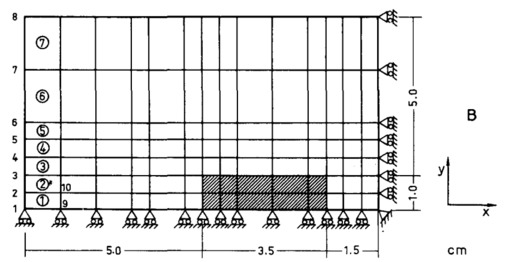
\includegraphics[height=4.5cm]{images/history/stbe71}\\
{\captionfont Model a boudinage structure - \textcite{stbe71} (1971)}
\end{minipage}\hfill
\begin{minipage}{0.45\textwidth}
\centering
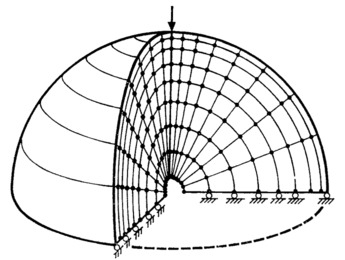
\includegraphics[height=4.5cm]{images/history/bela72}\\
{\captionfont Crustal Structure from Surface Load Tilts - \textcite{bela72} (1972)}
\end{minipage}
\end{center}


\begin{center}
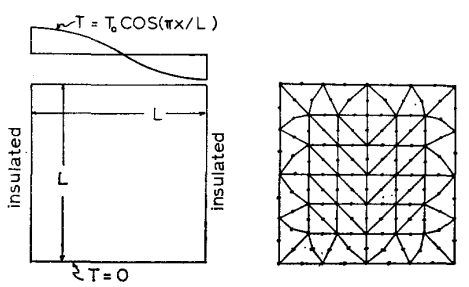
\includegraphics[height=5cm]{images/history/sath76}\\
{\captionfont Mantle convection in a square domain - \textcite{sath76} (1976)}
\end{center}

\begin{center}
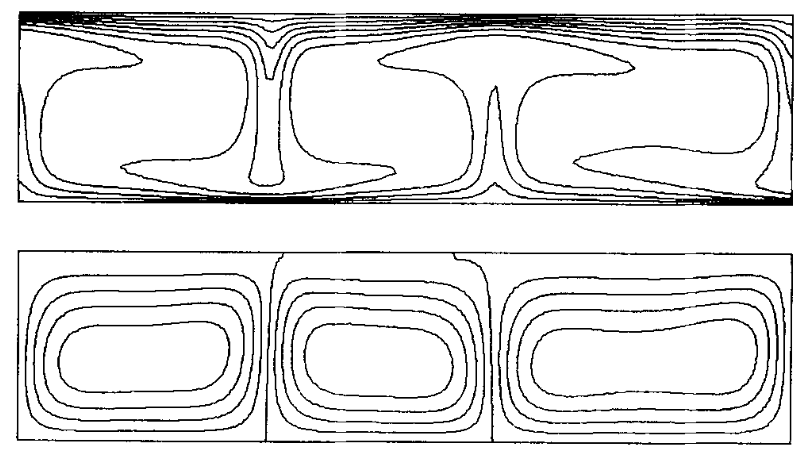
\includegraphics[height=4cm]{images/history/ludt79}\\
{\captionfont Mantle convection in a rectangular domain - \textcite{ludt79} (1979)}
\end{center}


\begin{center}
\begin{minipage}{0.45\textwidth}
\centering
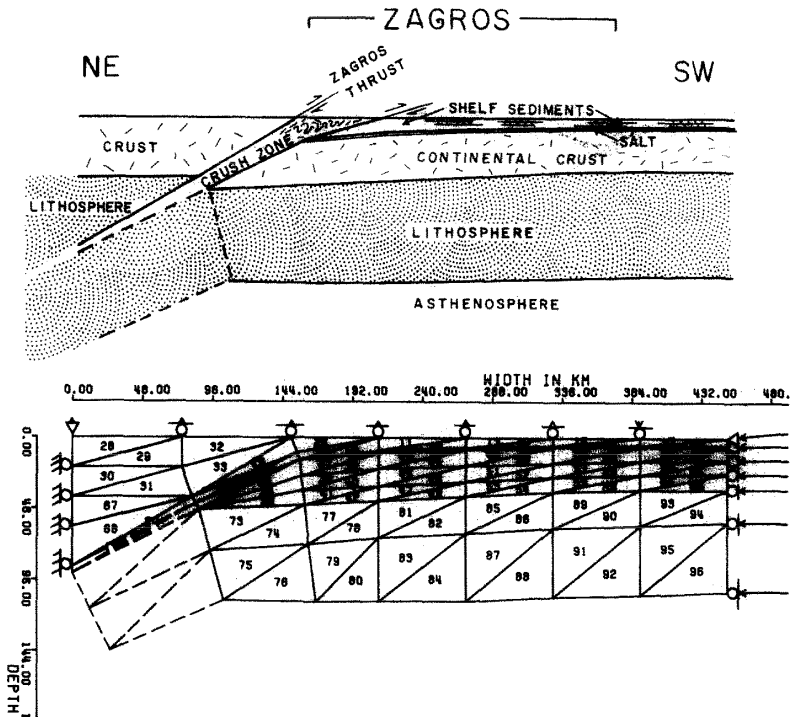
\includegraphics[height=5cm]{images/history/bird78b}\\
{\captionfont Finite element modelling of lithosphere deformation: the Zagros collision 
orogeny - \textcite{bird78b} (1978)}
\end{minipage}\hfill
\begin{minipage}{0.45\textwidth}
\centering
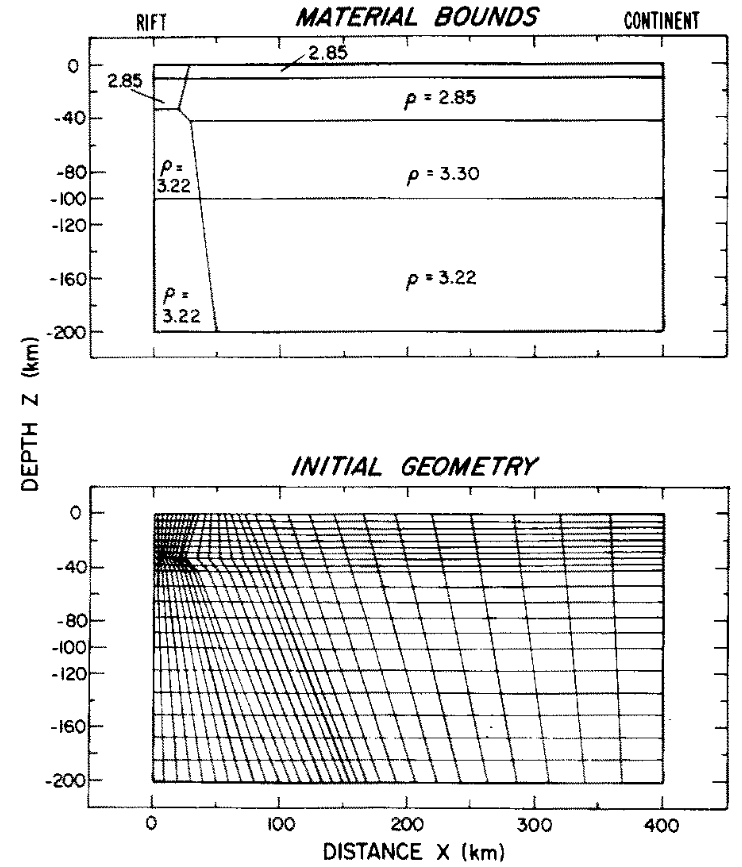
\includegraphics[height=5cm]{images/history/brpo81}\\
{\captionfont Thermal regimes, mantle diapirs and crustal stresses of 
continental rifts - \textcite{brpo81} (1981)}
\end{minipage}
\end{center}

\begin{center}
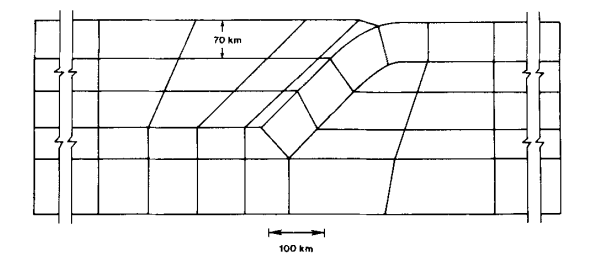
\includegraphics[height=3.5cm]{images/history/thar85}\\
{\captionfont Numerical models of subduction and forearc deformation - \textcite{thar85} (1985)}
\end{center}

\begin{center}
\begin{minipage}{0.48\textwidth}
\centering
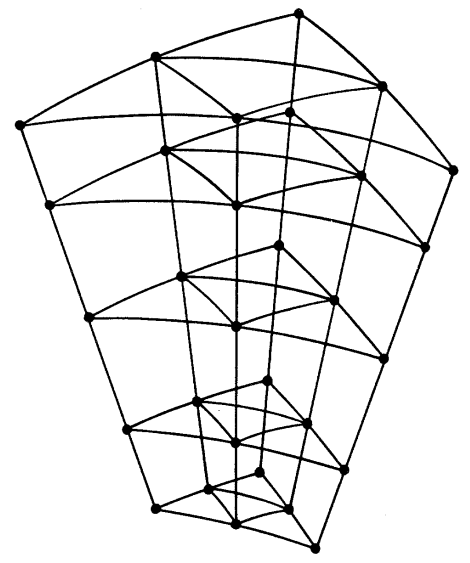
\includegraphics[height=3.5cm]{images/history/baum85a}
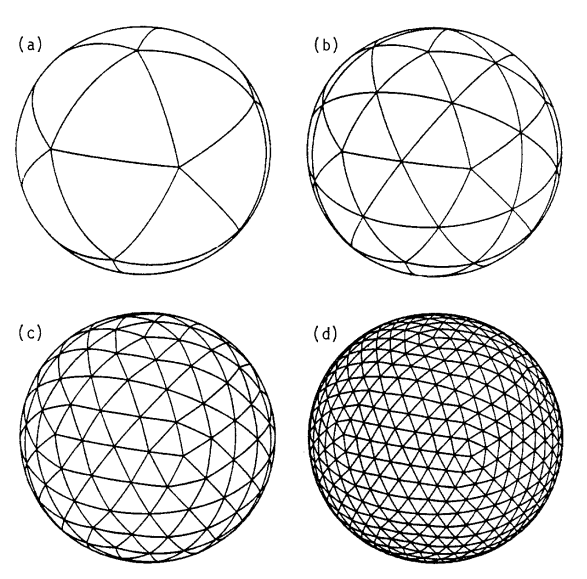
\includegraphics[height=3.5cm]{images/history/baum85b}\\
{\captionfont Three-Dimensional Treatment of Convective Flow in the Earth's Mantle -
\textcite{baum85} (1985)}
\end{minipage}\hfill
\begin{minipage}{0.45\textwidth}
\centering
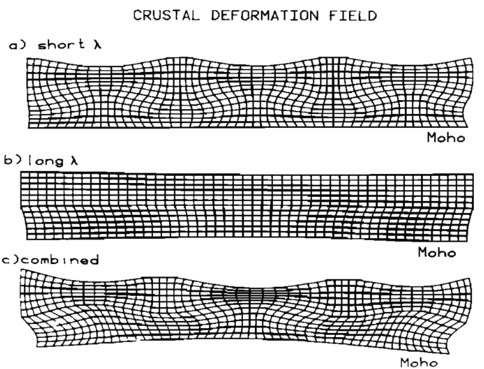
\includegraphics[width=7cm]{images/history/zupf86}\\
{\captionfont Lithospheric necking: a dynamic model for rift morphology - \textcite{zupf86} (1986)}
\end{minipage}
\end{center}


\begin{center}
\begin{minipage}{0.48\textwidth}
\centering
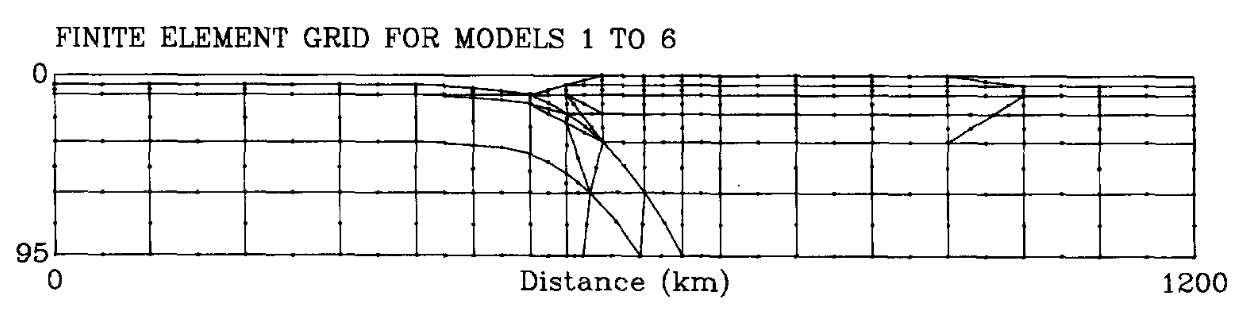
\includegraphics[width=9cm]{images/history/boww89}\\
{\captionfont Plate boundary forces at subduction zones and trench-arc compression - 
\textcite{boww89} (1989)}
\end{minipage}\hfill
\begin{minipage}{0.45\textwidth}
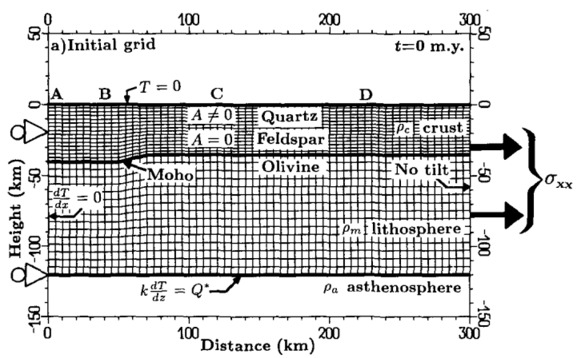
\includegraphics[width=9cm]{images/history/brbe89}\\
{\captionfont Relation between flank uplifts and the breakup unconformity at rifted continental 
margins - \textcite{brbe89} (1989)}
\end{minipage}
\end{center}



\begin{center}
\begin{minipage}{0.35\textwidth}
\centering
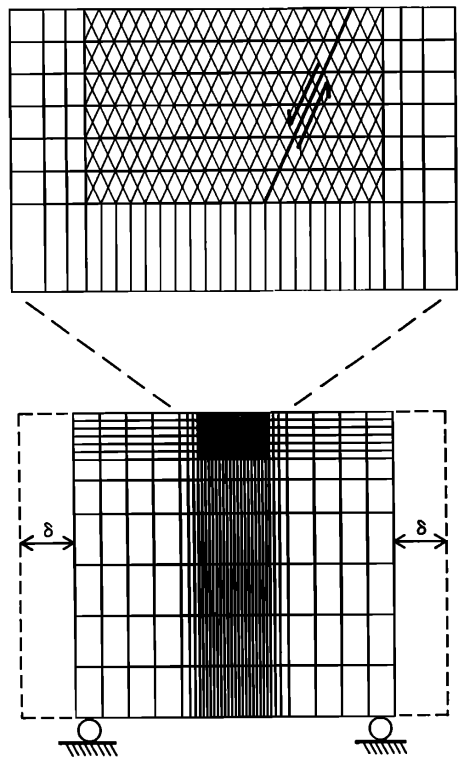
\includegraphics[width=5cm]{images/history/mewi89}\\
{\captionfont Mechanics of graben formation in crustal rocks - \textcite{mewi89} (1989)}
\end{minipage}\hfill
\begin{minipage}{0.55\textwidth}
\centering
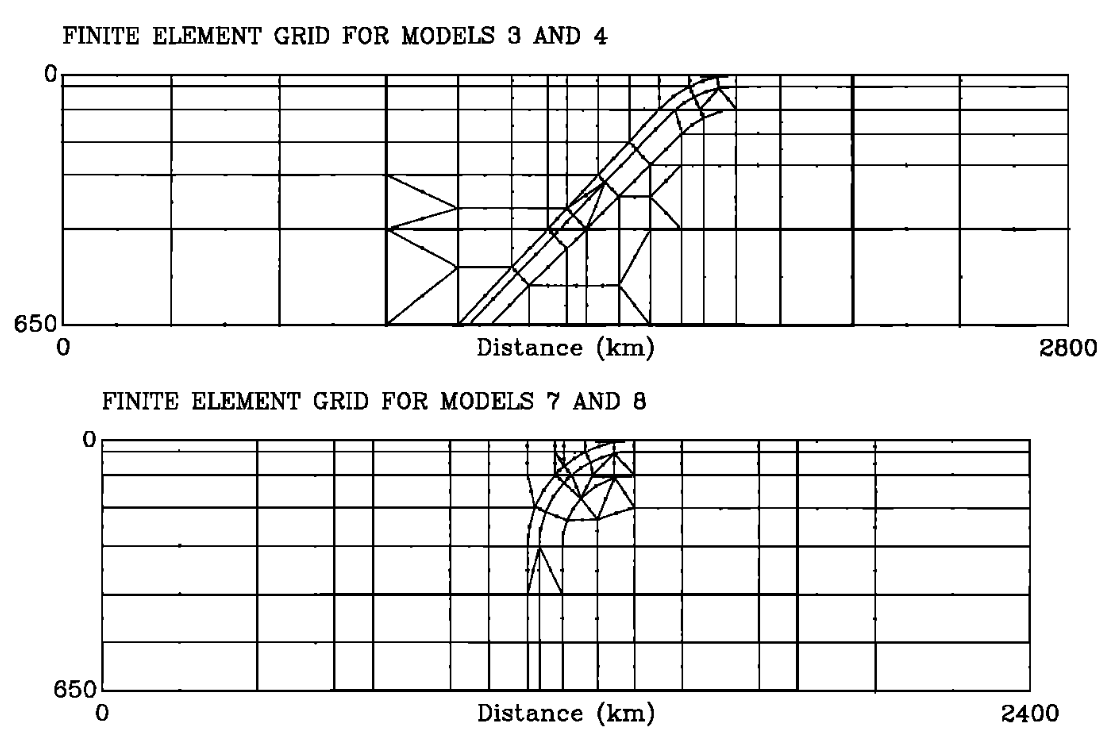
\includegraphics[width=8cm]{images/history/whbw92}\\
{\captionfont Stresses and plate boundary forces associated with subduction plate margins
- \cite{whbw92} (1992)}
\end{minipage}
\end{center}


\begin{center}
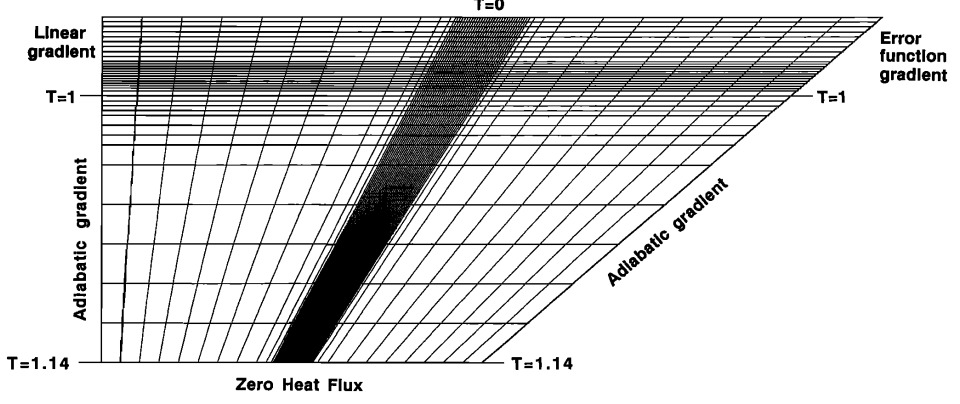
\includegraphics[width=5cm]{images/history/dast92}\\
{\captionfont Temperature field in subduction zones - \textcite{dast92} (1992)}
\end{center}


\begin{center}
\begin{minipage}{0.45\textwidth}
\centering
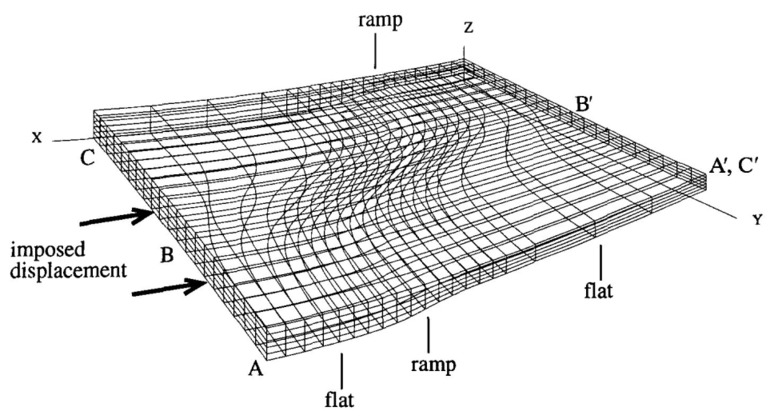
\includegraphics[width=7.6cm]{images/history/brau93}\\
{\captionfont 3D numerical modeling of
compressional orogenies: Thrust geometry and
oblique convergence - \textcite{brau93} (1993)}
\end{minipage}\hfill
\begin{minipage}{0.45\textwidth}
\centering
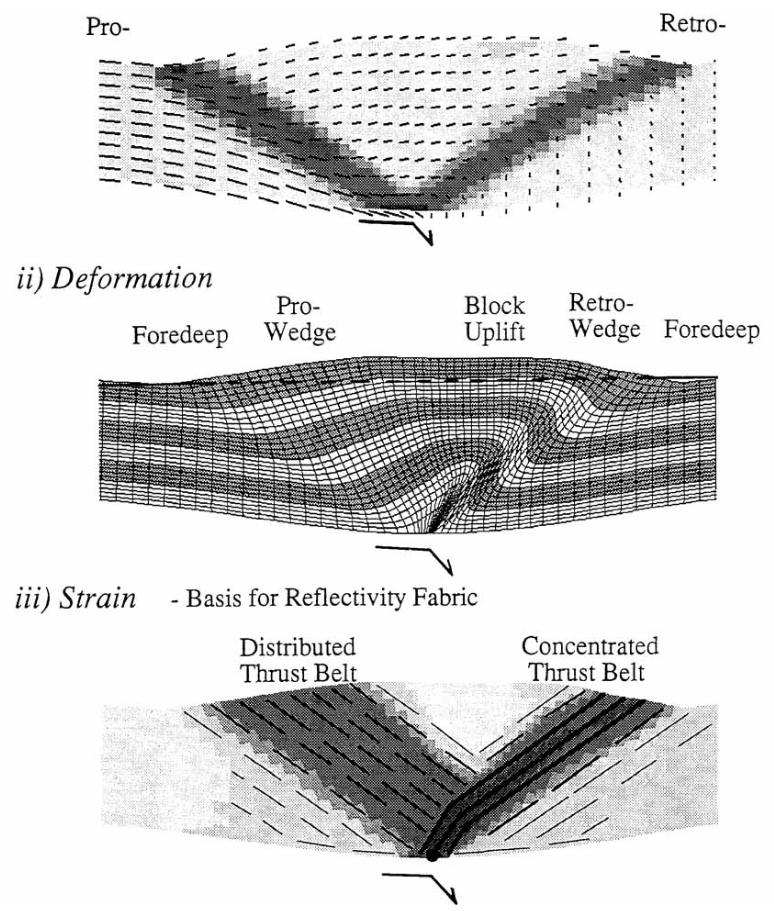
\includegraphics[height=6cm]{images/history/bequ94}\\
{\captionfont Crustal-scale compressional orogens - \textcite{bequ94} (1994)}
\end{minipage}
\end{center}

\begin{center}
\begin{minipage}{0.45\textwidth}
\centering
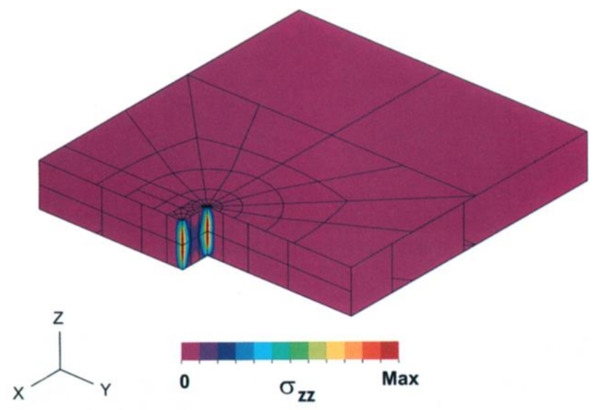
\includegraphics[height=6cm]{images/history/katl95}\\
{\captionfont Modeling of pull-apart basins - \textcite{katl95} (1995)}
\end{minipage}\hfill
\begin{minipage}{0.45\textwidth}
\centering
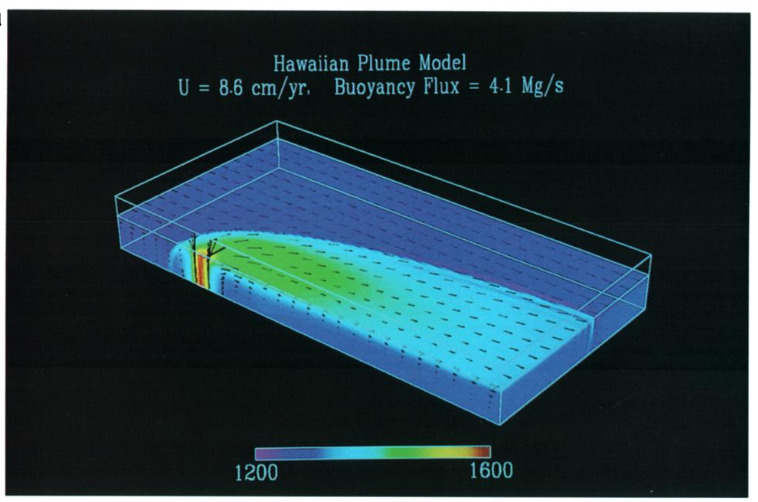
\includegraphics[height=6cm]{images/history/rich94}\\
{\captionfont Plume-lithosphere interaction - \textcite{rich94} (1994)}
\end{minipage}
\end{center}

\begin{center}
\begin{minipage}{0.45\textwidth}
\centering
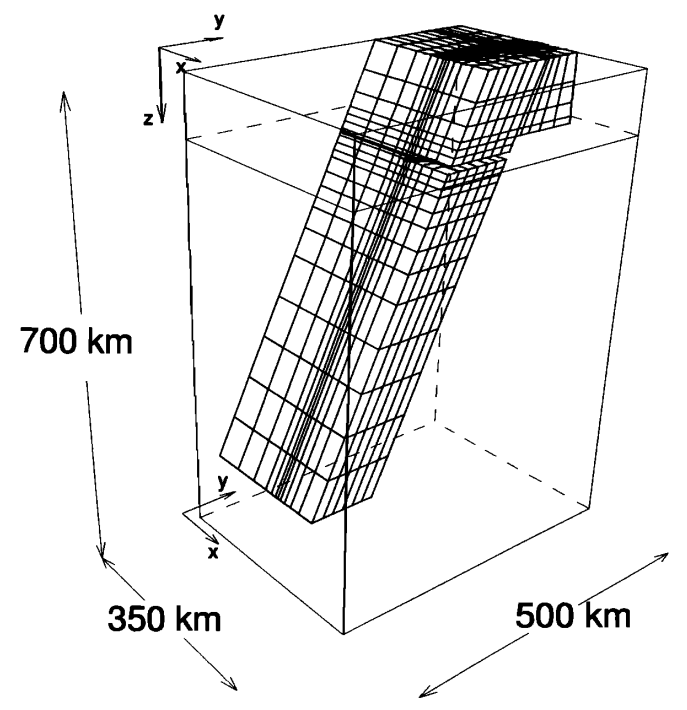
\includegraphics[height=5cm]{images/history/yowo95}\\
{\captionfont 3D numerical modeling of detachment of subducted 
lithosphere - \textcite{yowo95} (1995)}
\end{minipage}\hfill
\begin{minipage}{0.45\textwidth}
\centering
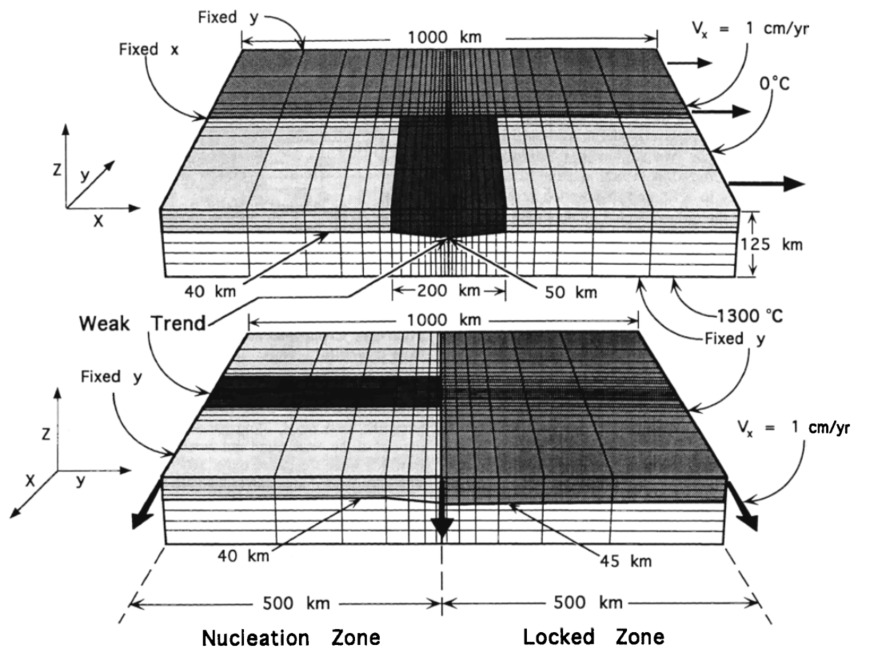
\includegraphics[height=6cm]{images/history/dusa96}\\
{\captionfont 3D dynamical model of continental rift propagation and 
margin plateau formation - \textcite{dusa96} (1996)}
\end{minipage}
\end{center}



\begin{center}
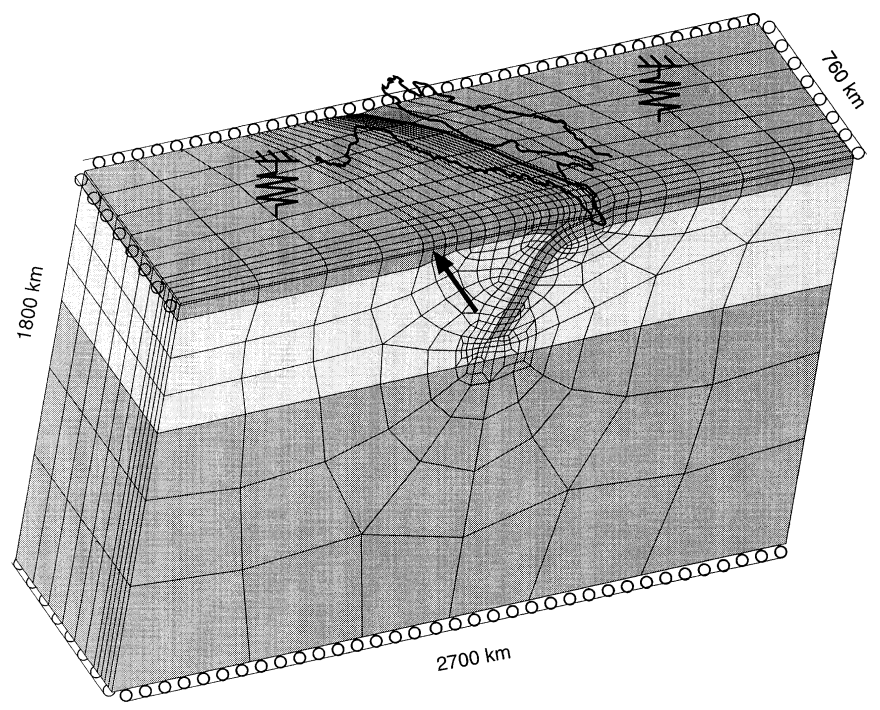
\includegraphics[height=6cm]{images/history/nesb99}\\
{\captionfont Model geometry, boundary conditions and 3-D finite element mesh used in 
the calculations. The circles denote a free-slip condition. The arrow denotes the velocity 
applied in some calculations to the southern boundary of the Tyrrhenian domain to simulate 
the motion of the African plate. The springs represent the buoyant restoring force applied 
at the surface - \textcite{nesb99} (1999)}
\end{center}

\Literature: 
\textcite{gart78} (1978), 
\textcite{anbr80} (1980), 
\textcite{mera80} (1980), 
\textcite{bran80} (1980),
\textcite{engl82} (1982),
\textcite{thar85} (1985), 
\textcite{scan85} (1985),
\textcite{enho86} (1986), 
\textcite{mofr86} (1986),
\textcite{zupa86} (1986), 
\textcite{boww89} (1989).




